\chapter{Freemind Example}
\label{ch:Freemind Example}

The example used for this paper is the \textit{automatic save file} feature of Freemind. Freemind is an open source  mind-mapping tool. The \textit{automatic save file} feature is a good example, because of it's name. Parts of the name are also mentioned in other features, which makes it slightly more difficult to only locate this specific feature.
A representiv callgraph of the important parts is shown in Fig 2.1.

\begin{wrapfigure}{r}{0.5\textwidth}
  \centering
  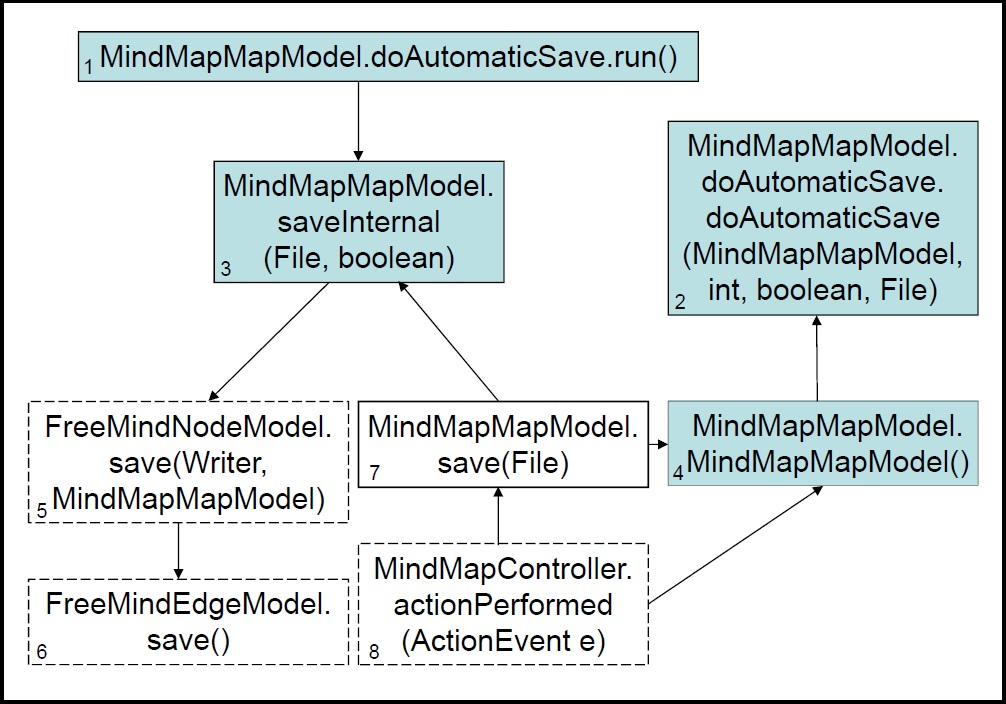
\includegraphics[width=\linewidth]{src/pic/freemind_callgraph}
  \label{dia:freemind callgraph}
  \caption{The Freemind callgraph \cite{FrM16} \cite{rubin2013survey}}
\end{wrapfigure}

As you can see here only the relevant constructors and methodsare shown and numbered with indices from 1 to 8. We reference them by using the number sign \# and then the corresponding number. Also the feature of the regarded function are highlighted with a blue background color. These are the methods which should be located if the \emph{automatic save file} function is the wanted feature. Note that the all the methods of different classes can in addition call other methods and constructors, which are irrelevant to the feature.
So as we can see the feature is mainly implemented by two methods of a subclass of \emph{MindMapMapModel} so called \emph{doAutomaticSave}:
\begin{itemize} 
\item the constructor, which is \#2. This constructor gets a few parameters to configurate the \emph{doAutomaticSave}-function and registers the class in the sheduling queue, so that it gets called.
\item the \emph{run()}-function \#1. This Methods gets called after the class is registered in the sheduling queue and everytime a special event is occurs. That can be different, like a period of time to shedule an automatic save or a preset number of actions within the main-programm. It calles the \emph{saveInternal}-method to do actual saveoperation.
\end{itemize}

Regarding the previously mentioned definition of a feature by Rajlich and Chen \ref{Rajlich_Chen}, we can now define the regarded feature as the following: \newline
\begin{tabular}{ r  l }
  name: & \emph{automatic save file}  \\
  intesion: & saves a file automaticly afer the occuring of an event\\
 extension: & \#1,  \#2, \#3 and \#4\\
\end{tabular}
The methods \#5 to \#8 aren't in the extension of the \emph{automaticSaveFile} feature.
Mainly \# 5 and \#6 are called by methods of the \emph{automaticSaveFile} feature, but aren't relevant to the specifies of this function.
\#7 and \#8 in fact call \#3 and \#4, but they handle a user triggered save-event, which obviously isn't important to the \emph{automaticSaveFile} feature.
\newline \newline
While all feature location techniques try to achive the same goal, which is the locating the feature extension to a given feature intension, they differate in the underlying base of assumptions they make to be able to get the tracebility. It will be declared more specific in chapter~\ref{ch:Classification and Methodology}. 
